\documentclass[12pt,dvipsnames]{beamer}
\geometry{paper=a6paper,landscape}

\usetheme{default}% I recommend
\usepackage[utf8]{inputenc}
\usepackage{utopia}
\usecolortheme{seahorse}
% \or\usetheme{Singapore}
% \or\usetheme{Boadilla}
% \or\usetheme{Pittsburgh}
% \or\usetheme{Madrid}
% \or\usetheme{Warsaw} % common choice, but often poor
% \fi

\usepackage{xcolor}
\usepackage{listings}
\usepackage{semantic}
\usepackage{graphicx,pgfplots,parskip}
\usepackage[utf8]{inputenc}
\usepackage[T1]{fontenc}
\usepackage{microtype}
\usepackage{amsmath}
\usepackage{amssymb}
\usepackage{ifthen}
\newcommand\hmmax{0} % default 3
% \newcommand\bmmax{0} % default 4
% \usepackage{bm}
\usepackage{stmaryrd}
\usepackage{proof}
\usepackage{graphicx}
\usepackage[export]{adjustbox}
\usepackage{listings}
\usepackage{tikz}
\usepackage{semantic}
\usepackage{setspace}
\usepackage{wrapfig}
\usepackage{caption}
\usepackage{subcaption}
\usepackage{esvect}
\usepackage{tikz}
\usepackage{booktabs} %% http://ctan.org/pkg/booktabs
\usepackage{wasysym}
\usepackage{array,multirow}
\usepackage{balance}
\usepackage{minted}
\usemintedstyle{tango}
\usepackage[backend=bibtex, style=authoryear-comp]{biblatex}
%%%%%%%%%%%%%%%%%%%%% MACROS %%%%%%%%%%%%%%%%%%%%%%%%%%%


\definecolor{lightgray}{gray}{0.9}
%\newcommand{\highlight}[1]{\colorbox{lightgray}{$\displaystyle #1$}}
\newcommand{\hi}[1]{\colorbox{lightgray}{$\displaystyle #1$}}

\newcommand{\tagsc}[1]{\tag{\textsc{#1}}}
\newcommand{\newname}[2]{\newcommand{#1}{\ensuremath{#2}}}

\newcommand{\overbar}[1]{\mkern 1.5mu\overline{\mkern-1.5mu#1\mkern-1.5mu}\mkern 1.5mu}

\newcommand{\size}{size}
\newcommand{\cast}{\Rightarrow}
\newcommand{\CoercionTyping}{\Longrightarrow}
\newcommand{\castE}[4][]{\ensuremathc{#2 : #3 \Rightarrow^{#1} #4}}

\newcommand{\key}[1]{\texttt{#1}}

% Types
\newcommand{\UnitT}{\ensuremath{\mathsf{()}}}
\newcommand{\IntT}{\ensuremath{\mathsf{Int}}}
\newcommand{\BoolT}{\ensuremath{\mathsf{Bool}}}
\newcommand{\DynT}{\ensuremath{\mathsf{\star}}}
\newcommand{\RefT}[1]{\ensuremath{\mathsf{Ref}\ #1}}
\newcommand{\RefPT}[1]{\ensuremath{\mathsf{Ref}\ #1}}
%\newcommand{\RefMT}[1]{\ensuremath{\mathsf{Ref}_m #1}}
\newcommand{\FunT}[2]{\ensuremath{#1 \to #2}}
\newcommand{\CFunT}[3]{\ensuremath{(\overbar{#1},#2) \cast #3}}
\newcommand{\PairT}[2]{\ensuremath{#1 \times #2}}
\newcommand{\Unit}{\ensuremath{\text{Unit}}}
\newcommand{\CClosT}[2]{\ensuremath{#1 \to #2}}
\newcommand{\CoT}[2]{\ensuremath{#1 \Longrightarrow #2}}

\newcommand{\IntC}{\ensuremath{\mathtt{Int}}}
\newcommand{\BoolC}{\ensuremath{\mathtt{Bool}}}
\newcommand{\DynC}{\ensuremath{\mathtt{Dyn}}}
\newcommand{\RefC}[1]{\ensuremath{\mathtt{Ref}\ #1}}

% Relations

\newcommand{\TypePreciseness}{\sqsubseteq}
\newcommand{\ExprTypePreciseness}{\sqsubseteq}
\newcommand{\StoreTypePreciseness}{\sqsubseteq_p}
\newcommand{\StoreTypeExtension}{\sqsubseteq_e}
\newcommand{\StoreTypeProgress}{\sqsubseteq_{p/e}}
\newcommand{\static}{\Rbag}
\newcommand{\ShallowConsist}{\small\smile}

% Coercions
\newcommand{\idC}{\ensuremath{\mathtt{\iota}}}
\newcommand{\InjectCoercion}[1]{\ensuremath{#1!}}
\newcommand{\seqInjC}[2]{\ensuremath{\seqC{#1}{\InjectCoercion{#2}}}}
\newcommand{\ProjectCoercion}[1]{\ensuremath{#1?}}
\newcommand{\seqPrjC}[2]{\ensuremath{\seqC{\ProjectCoercion{#1}}{#2}}}
\newcommand{\FunctionCoercion}[2]{\ensuremath{#1 \to #2}}
\newcommand{\RefCoercion}[1]{\ensuremath{\mathsf{Ref}\ #1}}
\newcommand{\seqC}[2]{\ensuremath{#1 \, ; \, #2}}
\newcommand{\FailCoercion}[2]{\ensuremath{\bot^{#1,#2}}}
\newcommand{\FailCoercionSE}{\ensuremath{\bot}}
\newcommand{\PairCoercion}[2]{\ensuremath{#1 \times #2}}

\newcommand{\coercion}[1]{\ensuremath{\langle #1 \rangle}}
\newcommand{\coerce}[2]{\ensuremath{#1 \coercion{#2}}}
\newcommand{\coerced}[2]{\ensuremath{\coerce{#1}{#2}}}
\newcommand{\app}[2]{\ensuremath{#1 \, #2}}
\newcommand{\lam}[2]{\ensuremath{\lambda #1 .\, #2}}
\newcommand{\blame}[1]{\ensuremath{\mathtt{blame}\, #1}}
\newcommand{\mkRef}[1]{\ensuremath{\mathtt{ref}\ #1}}
\newcommand{\allocT}[2]{\ensuremath{\mathtt{ref}\ #1 @ #2}}
\newcommand{\alloc}[1]{\allocT{#1}{\AllTa}}
\newcommand{\deref}[1]{\ensuremath{\mathtt{!} #1}}
\newcommand{\derefT}[1]{\ensuremath{\mathtt{!} #1 @ \AllTa}}
\newcommand{\DerefT}[2]{\ensuremath{\mathtt{!} #1 @ #2}}
\newcommand{\setref}[2]{\ensuremath{#1\ {:=}\ #2}}
\newcommand{\setrefT}[2]{\ensuremath{#1\ {:=}\ #2 @ \AllTa}}
\newcommand{\SetrefT}[3]{\ensuremath{#1\ {:=}\ #2 @ #3}}
\newcommand{\error}{\ensuremath{\mathtt{error}}}
\newcommand{\Error}{\ensuremath{\mathtt{Err}}}
\newcommand{\dom}[1]{\ensuremath{\text{dom}(#1)}}
\newcommand{\pair}[2]{\ensuremath{(#1,#2)}}
\newcommand{\fst}[1]{\ensuremath{(\mathtt{fst}\, #1)}}
\newcommand{\snd}[1]{\ensuremath{(\mathtt{snd}\, #1)}}

\newcommand{\glbt}{\sqcap}

\newcommand{\var}[1][x]{\ensuremath{#1}}
\newcommand{\expr}[1][e]{\ensuremath{#1}}
\newcommand{\const}{\ensuremath{k}}

\newcommand{\uncoerced}{\ensuremath{u}}
\newcommand{\val}{\ensuremath{v}}
\newcommand{\DelayedCastA}{\ensuremath{dc}}
\newcommand{\DelayedCastB}{\ensuremath{dc'}}
\newcommand{\DelayedCastC}{\ensuremath{dc''}}
\newcommand{\ReducibleDelayedCast}{\ensuremath{dc^{+}}}

\newcommand{\hole}{\ensuremath{\square}}
\newcommand{\context}[2]{\ensuremath{ #1 [ #2 ] }}

\newcommand{\InertCoercion}[1]{\ensuremath{#1\uparrow}}
\newcommand{\InertCoercionA}{\InertCoercion{\seCa}}
\newcommand{\InertCoercionB}{\InertCoercion{\seCb}}
\newcommand{\InertFinalCoercion}{\ensuremath{\seFinalC\uparrow}}
\newcommand{\InertMiddleCoercion}{\ensuremath{\seInterC\uparrow}}
\newcommand{\ActiveCoercion}[1]{\ensuremath{#1\downarrow}}
\newcommand{\ActiveCoercionA}{\ActiveCoercion{\seCa}}
\newcommand{\ActiveCoercionB}{\ActiveCoercion{\seCb}}
\newcommand{\ActiveFinalCoercion}{\ensuremath{\seFinalC\downarrow}}
\newcommand{\ActiveMiddleCoercion}{\ensuremath{\seInterC\downarrow}}

\newcommand{\CastCong}{\varphi}
\newcommand{\AllowCastCong}{\top}
\newcommand{\DisallowCastCong}{\bot}
\newcommand{\PureSymbol}{\obslash}
\newcommand{\ImpureSymbol}{\ocircle}
\newcommand{\PureCastReduce}{\longrightarrow_{c}^{\PureSymbol}}
% \newcommand{\PureCastDelayedCastReduce}{\longrightarrow_{dc}^{\PureSymbol}}
\newcommand{\PureCastDelayedCastReduce}{\longrightarrow}
\newcommand{\MonoCastReduce}{\longrightarrow_{c}^{\ImpureSymbol}}
\newcommand{\CastReduce}{\longrightarrow_{c}}
\newcommand{\DelayedCastReduce}{\longrightarrow_{dc}}
\newcommand{\PureReduce}{\longrightarrow_{e}^{\PureSymbol}}
\newcommand{\MonoReduce}{\longrightarrow_{e}^{\ImpureSymbol}}
\newcommand{\ProgReduce}{\longrightarrow_{e}}
\newcommand{\Lang}{\ensuremath{\textsc{GTLC}^{+}}}

% Meta Variables
\newname{\BaseT}{B}
\newname{\InjTa}{I}
\newname{\InjTb}{J}
\newname{\AllTa}{T}
\newname{\AllTb}{S}
\newname{\topC}{c}
\newname{\noFailC}{r}
\newname{\blameLabel}{p}
\newname{\addr}{a}
\newname{\seCa}{c}
\newname{\seCb}{d}
\newname{\ca}{c}
\newname{\cb}{d}
\newname{\seFinalC}{i}
\newname{\seInterC}{g}
\newname{\seIdFreeC}{f}
\newname{\CoercionT}{\mathcal{C}}
\newname{\expra}{M}
\newname{\exprb}{N}
\newname{\ctag}{w}
\newname{\uctag}{uc}
\newname{\cctag}{cc}

% Functions
\newcommand{\ComposeCoercion}{\fatsemi}
\newcommand{\ComposeMiddleCoercion}{\ensuremath{\fatsemi_{\text{\tiny g}}}}
\newcommand{\ComposeFinalCoercion}{\ensuremath{\fatsemi_i}}
\newcommand{\mkC}[2]{\ensuremath{ #1 \Rightarrow #2 }}

\newcommand{\jdgt}[2]{\ensuremath{\Gamma\vdash #1:#2}}
\newcommand{\ctit}[3]{\ensuremath{\Gamma\vdash #1 \hookrightarrow #2:#3}}
\newcommand{\mkCrcn}[2]{\ensuremath{\langle #1 \Longrightarrow #2
    \rangle}}

% Heaps
\newcommand{\store}{\ensuremath{\mu}}
\newcommand{\evstore}{\ensuremath{\nu}}
\newcommand{\storecell}[1]{\ensuremath{\addr \mapsto #1}}
\newcommand{\mstorecell}[2]{\ensuremath{\addr \mapsto #1 : #2}}
\newcommand{\StoreCell}[3]{\ensuremath{#1 \mapsto #2 : #3}}
\newcommand{\StoreValRead}{\ensuremath{\store(\addr)_{\text{val}}}}
\newcommand{\StoreRTTIRead}{\ensuremath{\store(\addr)_{\text{rtti}}}}
\newcommand{\EvStoreValRead}{\ensuremath{\evstore(\addr)_{\text{val}}}}
\newcommand{\EvStoreRTTIRead}{\ensuremath{\evstore(\addr)_{\text{rtti}}}}

\newcommand{\EvolvingStoreRTTIRead}[2]{\ensuremath{#1(#2)_{\text{rtti}}}}


\DeclareCiteCommand{\citeseries}
  {\usebibmacro{prenote}}
  {\usebibmacro{citeindex}%
    \printfield{series}}
  {\multicitedelim}
  {\usebibmacro{postnote}}

\addbibresource{all.bib}

\newcommand{\customcite}[1]{\citeauthor{#1}, \citetitle{#1},
  \citeseries{#1} \citeyear{#1}}

\newcommand{\customcitewithoutseries}[1]{\citeauthor{#1},
  \citetitle{#1}, \citeyear{#1}}

\lstdefinestyle{basic}{
%showstringspaces=false,
language=Python,
columns=fullflexible,
%basicstyle=\sffamily\small,%
basicstyle=\ttfamily,%
%columns=fixed,
%basewidth=0.49em,
%lineskip=0pt,
%escapechar=@,xleftmargin=1pc,%
keywordstyle=\ttfamily,
mathescape=true,%
moredelim=**[is][\color{blue}]{@}{@},
moredelim=[is][\color{red}]{|}{|},
moredelim=[is][\color{blue}]{~}{~},
%commentstyle=\rmfamily,%
%morekeywords={return,fix,var,proc,fun,func},%
%deletekeywords={int,bool}
}
\lstset{style=basic}

\newcommand{\lstsetgrift}{
  \lstset{%
    language=Lisp,
    numbers=left,
    stepnumber=1,
    basicstyle=\ttfamily\small,
    keywordstyle=\ttfamily\bfseries\small,
    columns=flexible,
    aboveskip=\smallskipamount,
    belowskip=\smallskipamount,
    xleftmargin=2pt,
    escapeinside={/+}{+/},
    mathescape=true,
    morekeywords=[1]{define,lambda,if,begin,letrec,let,let*,values,:,repeat,then,else,return,and,time,box,ref,unbox,box,ann},
    literate=
    {+}{{\textsf{+}}}1
    {-}{{\textsf{-}}}1
    {=>}{{$\rightarrow\;$}}2
    {lambda}{{$\boldsymbol{\lambda}$}}1
  }
}%%

\newcounter{stuff}
\newtheorem{prop}[stuff]{Proposition}

\title %optional
{Space-Efficient Monotonic References}
 
% \subtitle{A short story}
 
\author[Almahallawi, Siek] % (optional, for multiple authors)
{Deyaaeldeen Almahallawi \and Jeremy G. Siek}
 
\institute[IU] % (optional)
{
  \inst{}%
  Luddy School of Informatics, Computing, and Engineering\\
  Indiana University Bloomington
}
 
\date[WGT 2020] % (optional)
{Workshop on Gradual Typing, January 2020}

\begin{document}

\begin{frame}
\maketitle
\end{frame}

\begin{frame}{Outline}
\tableofcontents
\end{frame}

\section{Efficiency Challenges}

\begin{frame}{Outline}
  \tableofcontents[currentsection]
\end{frame}

\begin{frame}[fragile]{Chains of Proxies}
    \begin{center}
    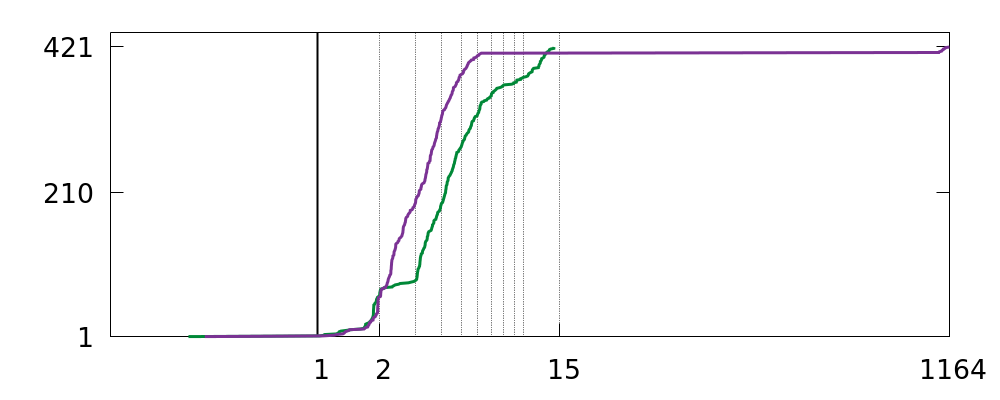
\includegraphics[scale=0.14]{plots/quicksort.png}
  \end{center}
  % \begin{itemize}
  % \item Soundness requires performing type checking at runtime.
  % \item Type checking for higher-order values create proxies that does
  %   checking at use sites.
  % \item A chain of proxies could be created if the same value crosses
  %   multiple boundaries.
  % \end{itemize}
\end{frame}

% \begin{frame}[fragile]{Dynamic Dispatch for Proxies}
%   \begin{itemize}
%   \item With proxies, use sites have to determine if the incoming value
%     is proxied.
%   \item If the value, is proxied, the checks carried by the proxy have
%     to be performed first before processing the value underneath.
%   \item This dynamic dispatch is performed even in statically-typed code.
%   \end{itemize}
% \end{frame}

% \begin{frame}[fragile]{Dynamic Dispatch For Reference Coercions}
% \begin{minipage}{.5\textwidth}
% \begin{lstlisting}
% (define (ref-read r)
%   (if |(proxied? r)|
%      (cast 
%        (ref-read (proxy-ref r))
%        (proxy-sourc r) 
%        (proxy-target r))
%      (read r)))
% \end{lstlisting}
% \end{minipage}%
% \begin{minipage}{.5\textwidth}
% \begin{lstlisting}
% (define (ref-write r v)
%   (if |(proxied? r)|
%      (ref-write (proxy-ref r) 
%                   (cast 
%                    v
%                    (proxy-target r) 
%                    (proxy-source r)))
%      (write r v)))
% \end{lstlisting}
%   \end{minipage}
% \end{frame}

\begin{frame}[fragile]{Dynamic Dispatch in Statically-typed Code}

\begin{lstlisting}
(define (partition [a : (Vect Int)] [p : Int] [r : Int]) : Int
    (let ([i (- p 1)]
           [x |(vector-ref a r)|])
      (repeat (j p r)
                (if (<= |(vector-ref a j)| x)
                    (begin
                      (set! i (+ i 1))
                      (swap a i j))
                    ()))
        (swap a (+ i 1) r)
        (+ i 1)))
(define (swap [a : (Vect Int)] [i : Int] [j : Int]) : Unit
    (if (= i j)
        ()
        (let ([t |(vector-ref a i)|])
          |(vector-set! a i (vector-ref a j))|
          |(vector-set! a j t)|)))
\end{lstlisting}
\end{frame}

\begin{frame}[fragile]{Solved?}
  \begin{center}
  \begin{tabular}{|c|cc|}
    \hline
    Problem/Feature & Functions & References \\
    \hline
    Chains of Proxies & \checkmark & \checkmark \\
    Dynamic Dispatch & \checkmark & \checkmark \\
    \hline
  \end{tabular}
\end{center}
\pause But, how to combine and implement them?
\end{frame}

\begin{frame}[fragile]{Solutions}
  \begin{center}
  \begin{tabular}{|c|cc|}
    \hline
    Problem/Feature & Functions & References \\
    \hline
    Chains of Proxies & Coercions\footnote[frame]{\customcite{Siek:2015ab}} & Monotonic\footnote[frame]{\customcite{Siek:2015aa}}/Coercions \\
    Dynamic Dispatch & Closure extension\footnote[frame]{\customcite{Siek:2012uq}} & Monotonic \\
    \hline
  \end{tabular}
\end{center}
\end{frame}

\begin{frame}[fragile]{Combination of Solutions}
  \begin{center}
  \begin{tabular}{|c|cc|}
    \hline
    Problem/Feature & Functions & References \\
    \hline
    Chains of Proxies & \textcolor{blue}{Coercions} & \textcolor{blue}{Monotonic}/Coercions \\
    Dynamic Dispatch & Closure extension & \textcolor{blue}{Monotonic} \\
    \hline
  \end{tabular}
\end{center}
\end{frame}

\begin{frame}[fragile]{Research Questions}
  \begin{center}
\begin{enumerate}
\item How to integrate monotonic references into a space-efficient
  coercion calculus?
\item How to implement monotonic references in a way that only puts
  values in the heap?
\end{enumerate}
\end{center}
\end{frame}

\section{Reviewing Monotonic References}

\begin{frame}{Outline}
  \tableofcontents[currentsection]
\end{frame}

\begin{frame}{Reviewing Monotonic References}
  \begin{center}
  \begin{itemize}
  \item Values are just addresses.
  \item $\forall \addr.\ s.t.\ \addr : \RefT{\AllTa}$, 
    $\Sigma(\addr) \TypePreciseness \AllTa$
  \item Stores expressions on the heap!
  \end{itemize}
  \vspace{0.5cm}
  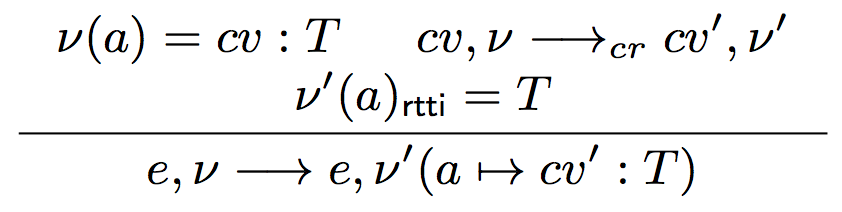
\includegraphics[scale=0.25]{rule.png}
  \end{center}
\end{frame}

\begin{frame}[fragile]{Reviewing Monotonic References (Cont'd)}
  \lstset {
    numbers=left,
    stepnumber=1
  }
\centering
\begin{center}
\begin{minted}
[
framesep=2mm,
baselinestretch=1.2,
bgcolor=lightgray,
fontsize=\footnotesize,
linenos,
escapeinside=||
,mathescape=true
]
{racket}
(: f Dyn)
(define f (lambda (x) x))
(: r Dyn)
(define r (box (cons f '())))
(set-box! r (cons f r)) ;; establish a cycle
(define (g [x : (Boxof (Pair (Dyn -> Integer)
                             (Boxof (Pair (Integer -> Dyn)
                                          Dyn))))])
  ((car (unbox x)) 42))
(g r)
\end{minted}
\end{center}
\end{frame}

\begin{frame}[fragile]{Old Work Writes Expressions to The Heap}
  \begin{center}
    Heap has
    $a \mapsto \pair{\coerced{(\lambda x. x)}{\FunT{\DynT}{\DynT}
        \cast \DynT}}{\coerced{a}{\RefT{(\PairT{\DynT}{\DynT})} \cast
        \DynT}}$
    \\
    \pause
    \vspace{0.5cm}
    $\addr$ should be cast to $\PairT{(\FunT{\DynT}{\IntT})}{\RefT{ (\PairT{
          (\FunT{\IntT}{\DynT}) }{ \DynT }) }}$
    \\
    \pause
    \vspace{0.5cm}
    {\huge{$\longrightarrow^{*}$}}
    \[
      a \mapsto
      \left\langle
        \begin{array}{l}
          {\coerced{\textcolor{RoyalPurple}{\coerced{(\lambda x. x)}{\FunT{\DynT}{\DynT} \cast \DynT}}}{\textcolor{Magenta}{\DynT \cast
          (\FunT{\DynT}{\IntT})}}}, \\
          {\coerced{\textcolor{RoyalPurple}{\coerced{a}{\RefT{(\PairT{\DynT}{\DynT})} \cast \DynT}}}{\textcolor{Magenta}{\DynT \cast
          \RefT{(\PairT{(\FunT{\IntT}{\DynT})}{\DynT}})}}} 
        \end{array}
      \right\rangle
    \]
    \\
    \pause
    \vspace{0.5cm}
    {\huge{$\longrightarrow^{*}$}}
    \[
      a \mapsto
      \left\langle
        \begin{array}{l}
          \textcolor{RoyalPurple}{\coerced{(\lambda x. x)}{\FunT{\DynT}{\DynT} \cast \FunT{\DynT}{\IntT}}}, \\
          \coerced{\textcolor{RoyalPurple}{\coerced{a}{\RefT{(\PairT{\DynT}{\DynT})} \cast \DynT}}}{\textcolor{Magenta}{\DynT \cast
          \RefT{(\PairT{(\FunT{\IntT}{\DynT})}{\DynT})}}}
        \end{array}
      \right\rangle
    \]
    \\
    \pause
    \vspace{0.5cm}
    Type of the heap cell should be $\PairT{ (\FunT{\IntT}{\IntT}) }{ \RefT{(\PairT{(\FunT{\IntT}{\DynT})}{\DynT})} }$
  \end{center}
\end{frame}

\begin{frame}[fragile]{Old Work Writes Expressions to The Heap (Cont'd)}
  \begin{center}
    \[
      a \mapsto
      \left\langle
        \begin{array}{l}
          \textcolor{RoyalPurple}{\coerced{(\lambda x. x)}{\FunT{\DynT}{\DynT} \cast \FunT{\DynT}{\IntT}}}, \\
          \coerced{\textcolor{RoyalPurple}{\coerced{a}{\RefT{(\PairT{\DynT}{\DynT})} \cast \DynT}}}{\textcolor{Magenta}{\DynT \cast
          \RefT{(\PairT{(\FunT{\IntT}{\DynT})}{\DynT})}}}
        \end{array}
      \right\rangle
    \]
    \\
    \vspace{0.5cm}
    Type of the heap should be $\PairT{ (\FunT{\IntT}{\IntT}) }{
      \RefT{(\PairT{(\FunT{\IntT}{\DynT})}{\DynT})} }$
    \\
    \pause
    \vspace{0.5cm}
    Eventually,
    \[
      a \mapsto
      \textcolor{RoyalPurple}{\left\langle
          \begin{array}{l}
            \coerced{\coerced{(\lambda x. x)}{\FunT{\DynT}{\DynT} \cast \FunT{\DynT}{\IntT}}}{ \FunT{\DynT}{\IntT} \cast \FunT{\IntT}{\IntT}}, \\
            a
          \end{array}
        \right\rangle}
    \]
  \end{center}
\pause How could this behavior be implemented efficiently in a runtime system?
\end{frame}

\section{Space-Efficiency and Implementable Semantics}

\begin{frame}{Outline}
  \tableofcontents[currentsection]
\end{frame}

\begin{frame}{Normal-form Monotonic Coercion}
\begin{gather*}
  \inference{\AllTa \TypePreciseness \AllTa_2}{\RefCoercion{\AllTa} : \RefT{\AllTa_1} \Longrightarrow
    \RefT{\AllTa_2}}
\end{gather*}
\\
\[
    \begin{array}{rcl}
      \RefCoercion{\AllTa}\ \ComposeCoercion\ \RefCoercion{\AllTa'}
                                        & = &
                                              \RefCoercion{(\AllTa \glbt
                                              \AllTa')} \qquad \text{if } \AllTa \sim
                                              \AllTa'  \\
      \RefCoercion{\AllTa}\ \ComposeCoercion\ \RefCoercion{\AllTa'}
                                        & = &
                                              \FailCoercionSE
                                              \qquad\qquad\qquad \text{ if } \AllTa \not\sim
                                              \AllTa'
    \end{array}
  \]

\begin{prop}{Coercion composition height is bounded}
  \begin{center}
    $\| \seCa \ComposeCoercion \seCb\| \leq \max (\| \seCa \|, \| \seCb
    \|)$
  \end{center}
\end{prop}
\end{frame}

\begin{frame}[fragile]{Implementable Dynamic Semantics}
  \pause
  \begin{center}
\begin{minted}
[
framesep=2mm,
fontsize=\footnotesize,
baselinestretch=1.2,
bgcolor=lightgray,
fontsize=\footnotesize,
linenos,
escapeinside=||
,mathescape=true
]
{C}
while (cast_queue_is_not_empty(mref_cast_q)) {
        u170_address = cast_queue_peek_address(mref_cast_q);
        u171_t1 = ((int64_t *)u170_address)[((intptr_t)0)];
        u172_t2 = cast_queue_peek_type(mref_cast_q);
        u173_t3 = (u4_types_greatest_lower_bound(u171_t1, u172_t2));
        cast_queue_dequeue(mref_cast_q);
        if ((u171_t1 == u173_t3)) {
          u1237_tmp_rco = ((intptr_t)1);
        } else {
          u1237_tmp_rco = ((intptr_t)0);
        };
        if ((!u1237_tmp_rco)) {
          u174_vi = ((int64_t *)u170_address)[((intptr_t)1)];
          u558_init_value = ((intptr_t)1);
          u559_alloc_id = u856_stack_alloc;
          ((int64_t *)u559_alloc_id)[((intptr_t)0)] = u558_init_value;
          u176_ret_id_ = u559_alloc_id;
          u560_init_value = ((intptr_t)0);
          u561_alloc_id = u857_stack_alloc;
          ((int64_t *)u561_alloc_id)[((intptr_t)0)] = u560_init_value;
          u177_ret_fvs = u561_alloc_id;
          u1238_tmp_rco = (u7_make_coercion(
              u171_t1, u173_t3,, u176_ret_id_,
              u177_ret_fvs));
          u175_cvi =
              (u160_apply_coercion(u174_vi, u1238_tmp_rco, ((intptr_t)0)));
          ((int64_t *)u170_address)[((intptr_t)0)] = u173_t3;
          ((int64_t *)u170_address)[((intptr_t)1)] = u175_cvi;
        } else {
          0;
        };
      }
\end{minted}
    \end{center}
\end{frame}

\begin{frame}[fragile]{Implementable Dynamic Semantics}
  \begin{center}
\begin{minted}
[
framesep=2mm,
baselinestretch=1.2,
bgcolor=lightgray,
fontsize=\footnotesize,
linenos,
escapeinside=||
,mathescape=true
]
{racket}
(while (mref-cast-queue-not-empty?)
          (let* ([address (mref-cast-queue-peek-address)]
                 [t1 (Mbox-rtti-read address)]                 
                 [t2 (mref-cast-queue-peek-type)]
                 [t3 (greatest-lower-bound t1 t2)])
            (mref-cast-queue-dequeue)
            (when (not (= t1 t3))
                   (let ([vi (Mbox-val-read address)]
                         [cvi (apply-cast vi t1 t3 #f)])
                     (Mbox-rtti-set! address t3)
                     (Mbox-val-set! address cvi)))))
\end{minted}
\end{center}
\end{frame}

\begin{frame}[fragile]{Example of Reduction Using New Dynamic Semantics}
  \begin{center}
    The heap is
    $a \mapsto \pair{\coerced{(\lambda x. x)}{\FunT{\DynT}{\DynT} \cast
        \DynT}}{\coerced{a}{\RefT{(\PairT{\DynT}{\DynT})} \cast \DynT}}$
    \\
    \vspace{0.5cm}
    $\coerced{\addr}{\PairT{(\FunT{\DynT}{\IntT})}{\RefT{(\PairT{(\FunT{\IntT}{\DynT})}{\DynT})}}}\longrightarrow
    \ ?$
    \\
    \pause \vspace{0.5cm}

    The heap becomes:
    $\addr \mapsto \pair{\coerced{\lambda x. x}{\FunT{\DynT}{\DynT}\cast
        \FunT{\DynT}{\IntT}}}{\addr}$
    and the queue
    \begin{tikzpicture}[
      scale=0.45,
      squarednode/.style={rectangle, draw=green!60, fill=green!5, very thick, minimum size=20mm},
      ]
      \node[squarednode] at (-1, 1) (cast){$(\addr, \PairT{(\FunT{\IntT}{\DynT})}{\DynT})$};
    \end{tikzpicture}
    \\
    \pause
    \vspace{0.5cm}
    Eventually, the heap becomes:
    $ \addr \mapsto\pair{\coerced{\lambda x. x }{\FunT{\DynT}{\DynT}
        \cast\FunT{\IntT}{\IntT}}}{\addr}$
  \end{center}
\end{frame}

\section{Preliminary Performance Analysis}

\begin{frame}{Outline}
  \tableofcontents[currentsection]
\end{frame}

\begin{frame}{Grift\footnote[frame]{\customcite{Kuhlenschmidt:2019aa}}}
  \begin{center}
    \includegraphics{grift.jpg}
  \end{center}
\end{frame}

\begin{frame}{Monotonic vs Proxied References on Statically-typed Code}
  \begin{center}
    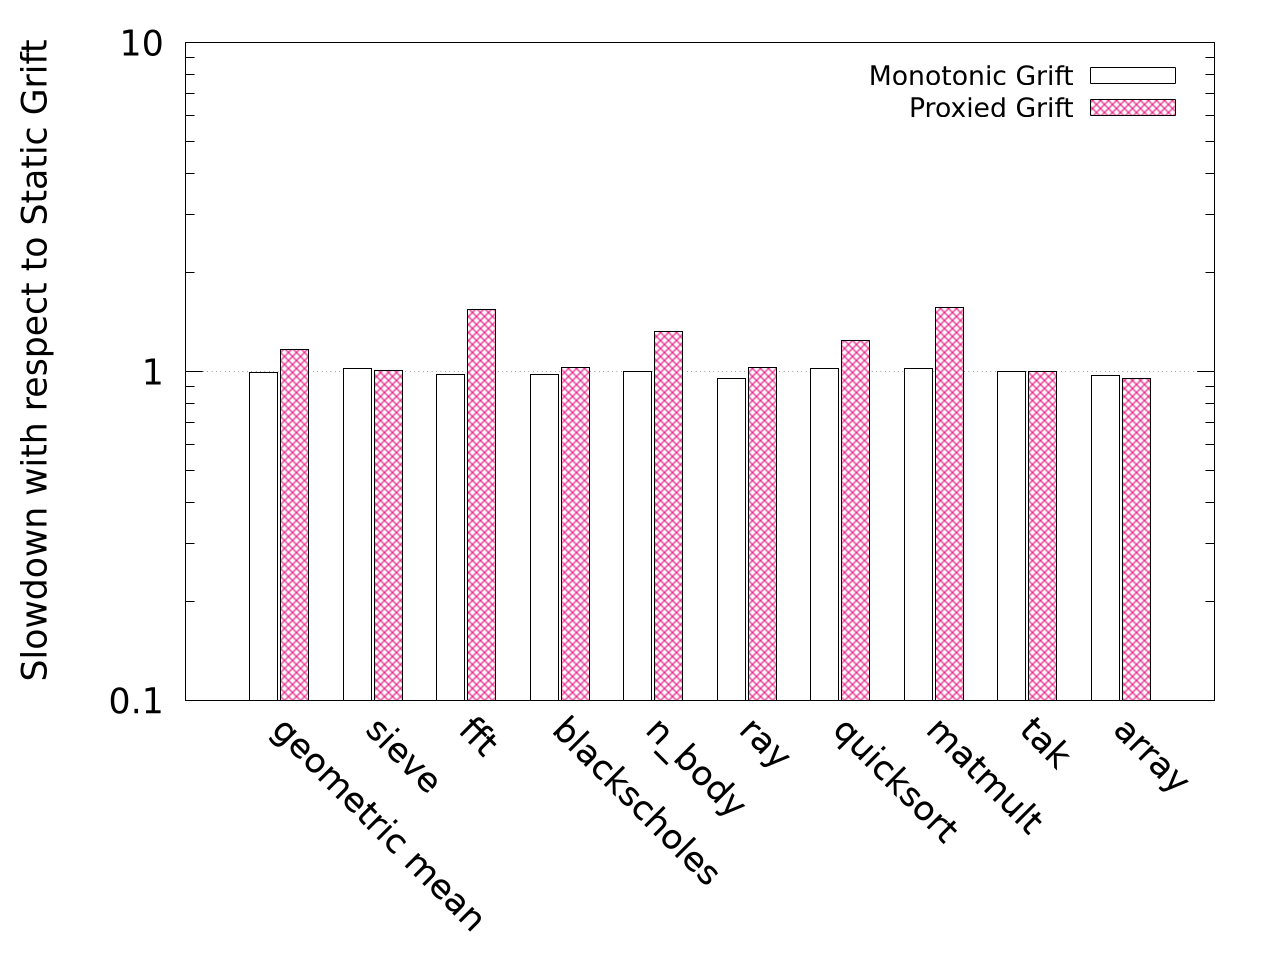
\includegraphics[scale=0.25]{plots/static.png}
  \end{center}
\end{frame}

\begin{frame}{Monotonic vs Proxied References on Mixed-typed Code}
  \begin{center}
    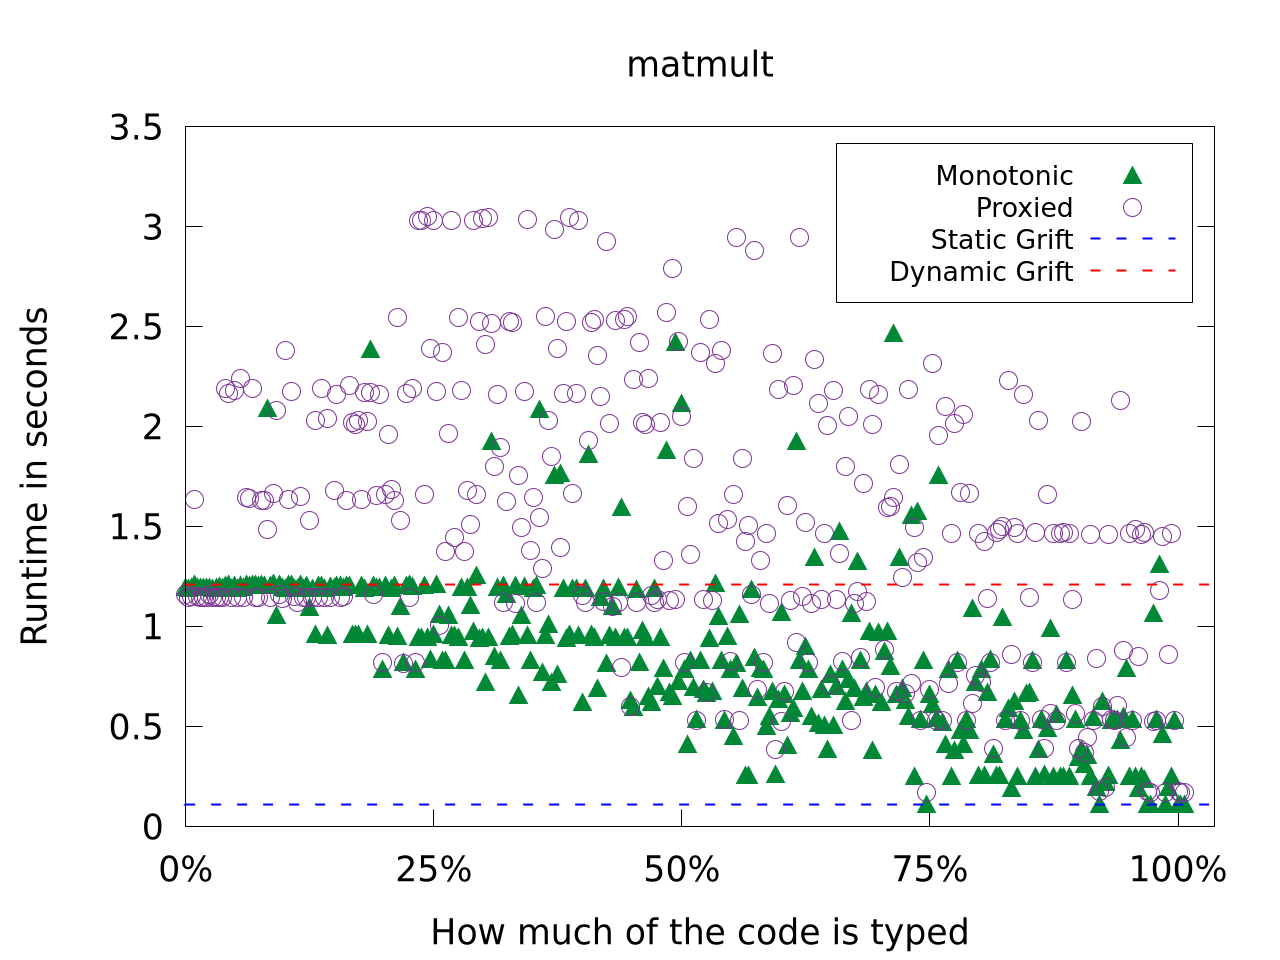
\includegraphics[scale=0.25]{plots/fine/Specialized_Coercions_Lazy/runtimes/matmult.png}
  \end{center}
\end{frame}

% \begin{frame}{Monotonic vs Proxied References on Mixed-typed Code (Cont'd)}
%   \begin{center}
%     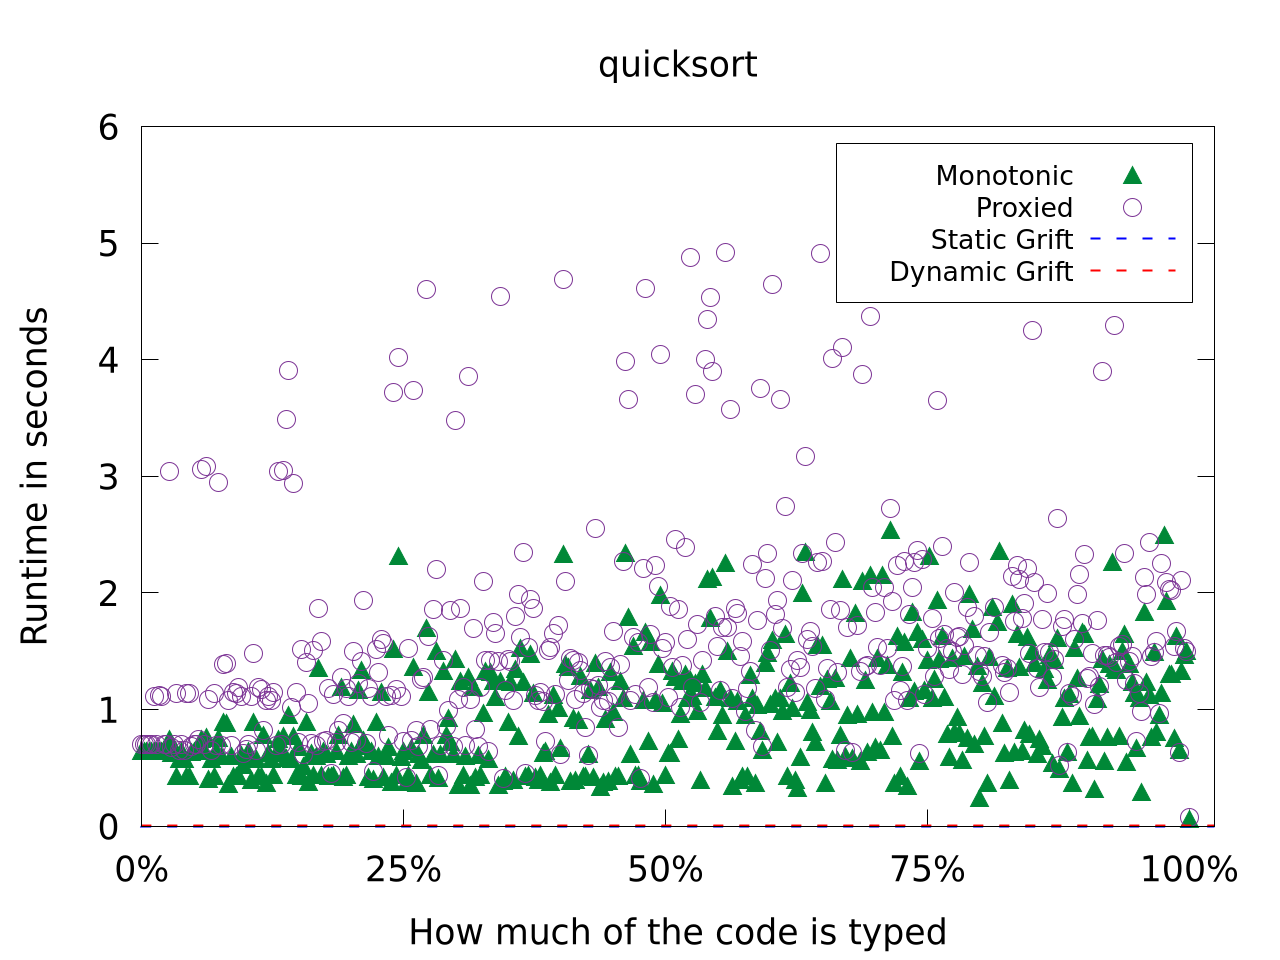
\includegraphics[scale=0.25]{plots/fine/Specialized_Coercions_Lazy/runtimes/quicksort.png}
%   \end{center}
% \end{frame}

\begin{frame}{Monotonic vs Proxied References on Mixed-typed Code (Cont'd)}
  \begin{center}
    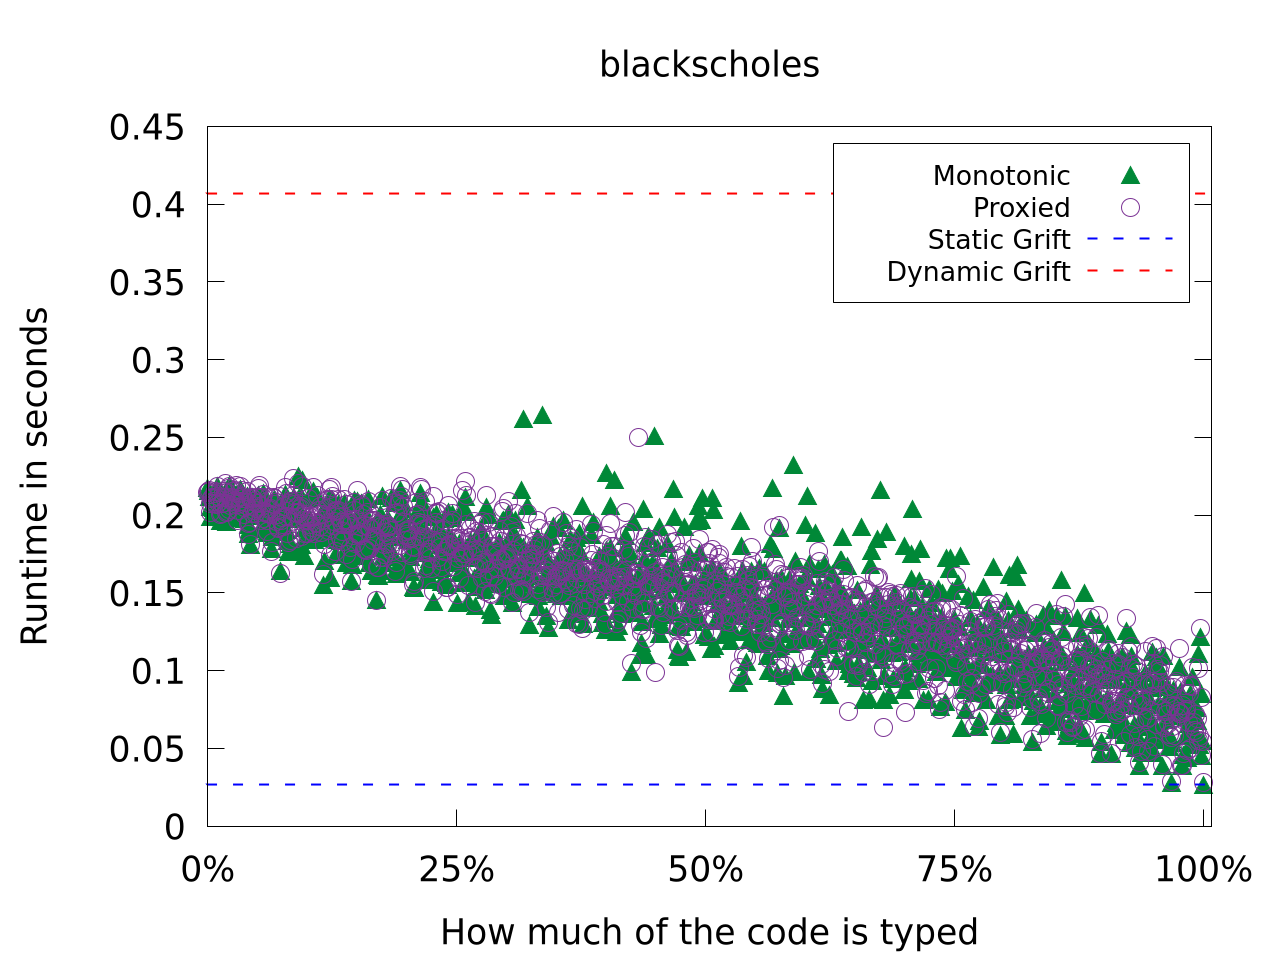
\includegraphics[scale=0.25]{plots/fine/Specialized_Coercions_Lazy/runtimes/blackscholes.png}
  \end{center}
\end{frame}

\begin{frame}{Conclusion}
  \begin{itemize}
  \item Proxies cause overheads in statically-typed code regions.
  \item Monotonic references eliminate these overheads but it was not
    obvious how to implement them in a runtime system.
  \item To achieve efficiency in both statically-typed and mixed-typed
    code regions, we integrate monotonic references into a
    space-efficient calculus based on coercions and provide dynamic
    semantics that is straightforward to implement.
  \end{itemize}
  \vspace{1cm}
  \centering
  Mechanized Formalism: \url{https://github.com/deyaaeldeen/monotonic}
  Implementation in Grift: \url{https://github.com/Gradual-Typing/Grift}
  \\
  \vspace{1cm}
  \centering
  \Huge Thank you!
\end{frame}

\end{document}

%%% Local Variables:
%%% mode: latex
%%% TeX-master: t
%%% End:
